\section{Appendix}
\label{app:appendix}
% \subsection{Comparison to Other Attribute-Masking strategies}
% \label{app:comparison}


\begin{table}[htbp]
    \centering
    \caption{Comparison with other attributed-masking methods in node classification. ``FT" means finetuning the model in downstream tasks, while ``LP" represents training a linear classifier for classification.}
    \begin{threeparttable}
    \begin{tabular}{c|ccc|c}
        \toprule[1.2pt]
                     & Cora     & Citeseer   & PubMed  & Type   \\
        \midrule
        GAE          & 71.5 &   65.8    & 72.1 & LP \\
        GPT-GNN      &  80.1    & 68.4 &     76.3       & LP \\
        NodeProp     &  81.94   &  71.60     &  79.44   & FT \\
        RASSL-GCN$^{1}$    &  83.80   &  72.95     & *81.23   & FT \\
        GATE         &  83.2    &  71.8      &  80.9    &  LP    \\
        \midrule
        \model       & 84.16    & 73.35      & 81.10    & LP  \\
        \bottomrule[1.2pt]
    \end{tabular}
            \begin{tablenotes}
            \footnotesize
            \item[1] PubMed dataset used is different from that in other baselines.
        \end{tablenotes}
    \end{threeparttable}
    \label{tab:com_attm}
\end{table}


\subsection{Results in the PPI Dataset}
\label{app:ppi}
Figure \ref{fig:ppi_hidden} shows the results of self-supervised learning methods in PPI dataset. Previous studies often report a large gap between supervised and self-supervised results on PPI. We find that increasing the number of model parameters helps little in supervised setting, but could highly boost the performance in self-supervised setting. As the hidden size reaches 2048$\times$4, \model even outperforms supervised counter-part, although the model would be too much larger. At least, this indicates that the gap could be filled.
% and \model benefits more from the larger model scale. 

The results of BGRL and GRACE in PPI are a bit different from those reported in ~\cite{thakoor2021bootstrapped}. This is because we train the linear classifier until convergence during evaluation, using the authors’ official code. In ~\cite{thakoor2021bootstrapped}, the classifier is trained only for a small fixed number of epochs, and the training does not converge.
% This might indicate the potential of large-scale GNNs in pre-training.



\begin{table}[htbp]
\centering
\caption{Experiment results using different encoder backbones in node classification.}
\renewcommand\tabcolsep{3pt}
\begin{tabular}{c|cccc}
\toprule[1.2pt]
          & Cora & Citeseer & Pubmed & Ogbn-arxiv \\
\midrule
BGRL (GCN)    &   82.7$\pm$0.6    &  71.1$\pm$0.7        & 79.4$\pm$0.6       &  71.64$\pm$0.12      \\
BGRL (GAT)    &   82.8$\pm$0.5    &   71.1$\pm$0.8       &  79.6$\pm$0.5      &   70.07$\pm$0.02 \\
CCA-SSG (GCN) &   84.0$\pm$0.4      &  73.1$\pm$0.3         &  81.0$\pm$0.4        &  70.81$\pm$0.13  \\
CCA-SSG (GAT) &   83.8$\pm$0.5    &  72.6$\pm$0.7        &   79.9$\pm$1.1     &  71.24$\pm$0.20  \\
\model (GCN)  &   82.9$\pm$0.6             &  72.5$\pm$0.5                 &  81.0$\pm$0.5               &  \bf 71.87$\pm$0.21\\   
\model (GAT)  &   \bf 84.2$\pm$0.4        &  \bf 73.4$\pm$0.4       & \bf 81.1$\pm$0.4      &  71.75$\pm$0.17 \\
\bottomrule[1.2pt]
\end{tabular}
\vspace{-2mm}
\label{tab:backbone}
\end{table}

\subsection{Ablation on the Encoder Architecture}
% \vpara{Effect of encoder architecture.}  
In node classification, \model uses GAT as the encoder. To have a fair comparison and investigate the influence of different GNN backbones, we compare the best baselines, BGRL and CCA-SSG, in node classification datasets using GCN and GAT as the encoder. The results are shown in Table \ref{tab:backbone}. We observe that \model still outperforms the baselines with the same GAT backbone. 
In addition, the results manifest that attention mechanism would not always benefit graph self-supervised learning, as GCN is inferior to GAT, for instance, in (Cora, CCA-SSG) and (Ogbn-arxiv, \model). Under the training setting of \model, GAT could be a better option in most cases.





\subsection{Implementation Details}
\subsubsection{Environment}
Most experiments are conducted on Linux servers equipped with an Intel(R) Xeon(R) CPU E5-2680 v4 @ 2.40GHz, 256GB RAM and NVIDIA 2080Ti GPUs. Experiments of Ogbn-arxiv and Reddit for node classificatin are conducted on Intel(R) Xeon(R) Gold 6240 CPU @ 2.60GHz and NVIDIA 3090 GPUs, as they require large memory. Models of node and graph classification are implemented in PyTorch version 1.9.0, DGL version 0.7.2 (\textit{\url{https://www.dgl.ai/}})  with CUDA version 10.2, scikit-learn version 0.24.1 and Python 3.7. 
% Our code and datasets will be available. 
For molecular property prediction, we implement our model based on the code in \textit{\url{https://github.com/snap-stanford/pretrain-gnns}} with Pytorch Geometric 2.0.4 (\textit{\url{https://www.pyg.org/}}).


\begin{figure}[htbp]
    \centering
    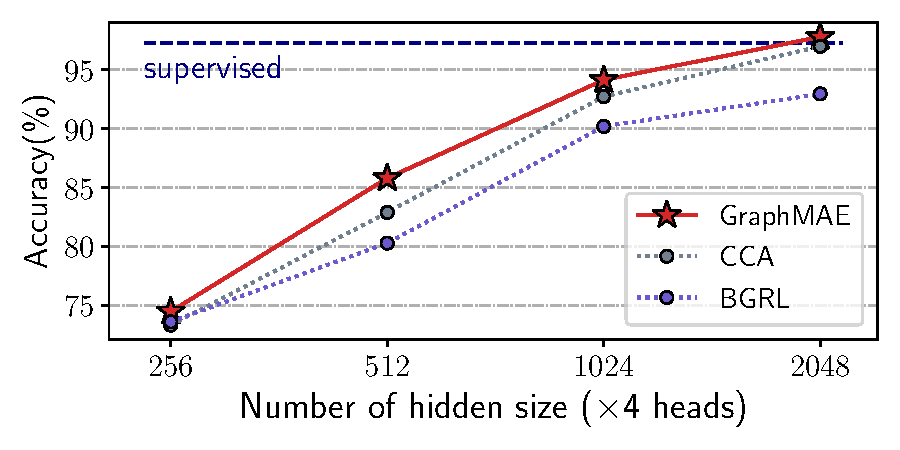
\includegraphics[width=0.37\textwidth]{imgs/ppi_hidden.pdf}
    \caption{Performance on PPI using GAT with 4 attention heads, compared to other baselines. Self-supervised methods benefit much from larger model size, and \model could outperform supervised model. }
    \label{fig:ppi_hidden}
\end{figure}


\begin{figure}[htbp]
    \centering
    \begin{minipage}{0.23\textwidth}
        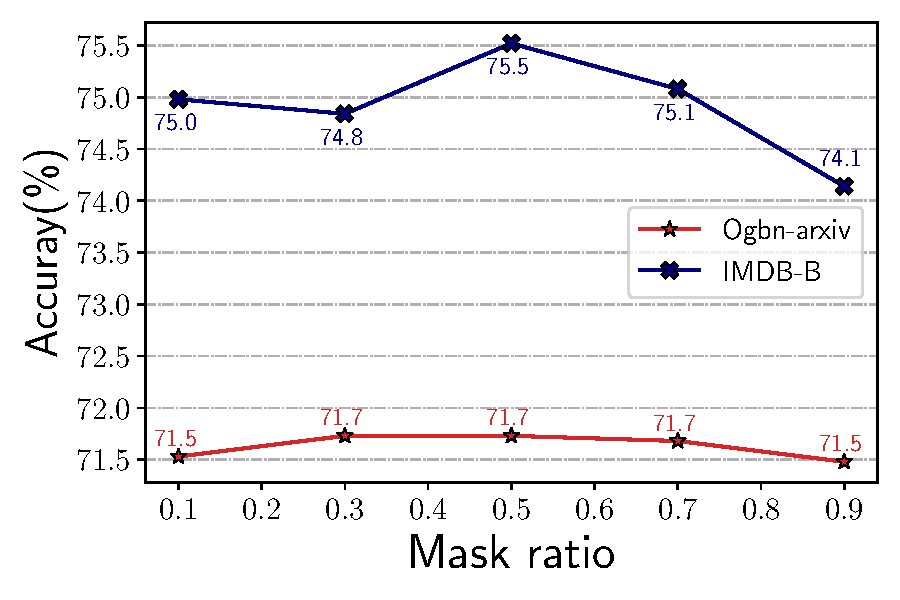
\includegraphics[width=\textwidth]{imgs/gmae_mask_ratio_append.pdf}
    \end{minipage}
    \begin{minipage}{0.23\textwidth}
        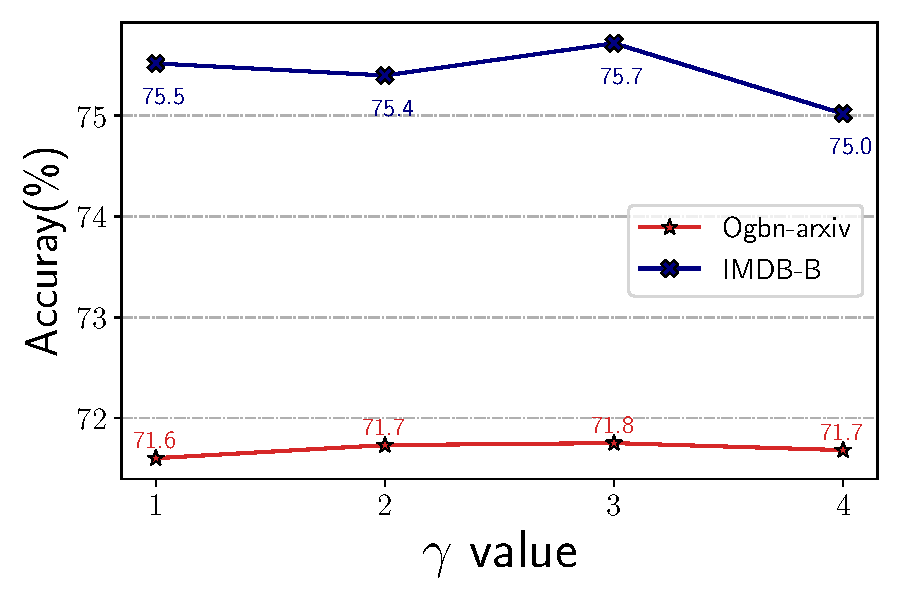
\includegraphics[width=\textwidth]{imgs/gamma_value_append.pdf}
    \end{minipage}
    \caption{Ablation study of mask ratio and scaling factor $\gamma$ in Ogbn-arxiv and IMDB-B.}
    \label{fig:abl_append}
\end{figure}

\hide{
\subsubsection{Model Configuration}
For node classification, we train the model using Adam Optimizer with $\beta_1 = 0.9, \beta_2 = 0.999, \epsilon = 1 \times 10^{-8}$. The initial learning rate is set to 0.001, using cosine learning rate decay without warmup. We use PReLU as the non-linear activation. More details about hyper-parameters and datasets are in Table \ref{tab:hp_node} and \url{https://github.com/THUDM/GraphMAE}.

For graph classification, we set the initial learning rate to 0.00015 with cosine learning rate decay for most cases. For the evaluation,  the parameter C of SVM is searched in the sets $\{10^{-3},...,10\}$. The hyper-parameters and statistics of datasets are in Table ~\ref{tab:hp_graph}.

For transfer learning of molecule property prediction, we adopt a single-layer GIN as decoder, the mask rate is set to 0.25, and we pretrain the whole model for 100 epochs.
% we implement the pre-training and finetune based on the code in \textit{\url{https://github.com/snap-stanford/pretrain-gnns}}.
% For the pre-training, 
For the finetuning, an Adam optimizer (learning rate: 0.001, batch size: 32) is employed to train the model for 100 epochs. We utilize a learning rate scheduler with fix step size, which multiplies the learning rate by 0.3 every 30 epochs for BACE only. Table ~\ref{tab:stat_mol} shows the statistics of datasets.
% for pre-training and finetune.



\subsection{Baselines}
% For GAT, GATE, DGI, and InfoGCL, we use the results reported in the previous papers. MVGRL's results are from DGL' reproducing. For GPT-GNN, GRACE, BRGL, and CCA-SSG, as they didn't report 
For node classification, the results of supervised baselines of GCN in Reddit, and GAT in Ogbn-arxiv and Reddit are from CogDL(\textit{\url{https://cogdl.ai/}}) if not reported before. For unsupervised baselines, GRACE~\cite{zhu2020deep}, BGRL~\cite{thakoor2021bootstrapped}, CCA-SSG~\cite{zhang2021canonical} are state-of-the-art contrastive learning methods in graph. 
% They did not report results in several benchmarks in their paper. 
GRACE and BGRL did not report the results in Cora, Citeseer, and PubMed of the public split. To have a fair comparison, we download the public source code and use the same GNN backbone as \model. We conduct hyper-parameter search for them and select the best results on the validation set.
% if the hyper-parameters are not provided in their repository.
The results of CCA-SSG are the output of the official code after the bugs in the code are fixed. For MVGRL~\cite{hassani2020contrastive}, we adopt DGL's reproducing results. We implement GPT-GNN~\cite{hu2020gpt} based on the official code for homogeneous networks, as the code is for heterogeneous networks, and report the results in Cora, Citeseer, and PubMed. 
% The sources of the codes used are as follows:
% \begin{itemize}
%     \item BRGL: \url{https://github.com/Namkyeong/BGRL_Pytorch}
%     \item GRACE: \url{https://github.com/CRIPAC-DIG/GRACE}
%     \item CCA-SSG: \url{https://github.com/hengruizhang98/CCA-SSG/}
%     \item MVGRL: \url{https://github.com/hengruizhang98/mvgrl}
%     \item GPT-GNN: \url{https://github.com/acbull/GPT-GNN}
% \end{itemize}

For graph classification and transfer learning of molecular property prediction, we adopt the results reported in previous papers if available. For the results of GraphCL~\cite{you2020graph} and JOAO~\cite{you2021graph} in IMDB-MULTI, we download the authors' official codes and keep hyper-parameters the same to get the output. }




\begin{table*}[htbp]
\centering
\label{tab:graph_sta_hyper}
\caption{Statistics and hyper-parameters for node classification datasets. ``s'' represents multi-class classification, and ``m'' means multi-label classification. 
% ``LN'' means layer-normalization.
}
\renewcommand\tabcolsep{6.5pt}
\renewcommand\arraystretch{1.05}
\begin{tabular}{c|c|cccccc}
\toprule[1.2pt]
& Dataset               & Cora & Citeseer & PubMed & Ogbn-arxiv & PPI       & Reddit    \\
\midrule
\multirow{3}{*}{Statistics}
&         \# nodes   & 2,708 & 3,327 & 19,717 & 169,343      & 56,944  & 232,965      \\
&         \# edges   & 5,429 & 4,732 & 44,338 & 1,166,243    & 818,736 & 11,606,919   \\
&         \# classes & 7(s)  & 6(s)  & 3(s)   & 40(s)        & 121(m)  & 41(s)         \\
\midrule
\multirow{6}{*}{Hyper-parameters} 
& scaling factor $\gamma$ & 3    & 1        & 3      & 3          & 3         & 3         \\
& masking rate            & 0.5  & 0.5      & 0.75   & 0.5        & 0.5       & 0.75      \\
& replacing rate          & 0.05 & 0.10     & 0      & 0          & 0         & 0.15      \\
& hidden\_size            & 512  & 512      & 1024   & 1024       & 1024      & 512       \\
% & num\_layer              & 2    & 2        & 2      & 3          & 3         & 4         \\
& weight\_decay           & 2e-4 & 2e-5     & 1e-5   & 0          & 0         & 2e-4      \\
& max\_epoch              & 1500 & 300      & 1000   & 1000       & 1000      & 500       \\
% & Norm                    & -    & -        & -      & LN  & LN & LN \\
\bottomrule[1.2pt]
\end{tabular}
\label{tab:hp_node}
\end{table*}



% Please add the following required packages to your document preamble:
% \usepackage{multirow}
\begin{table*}[htbp]
\centering
\label{tab:node_sta_hyper}
\caption{Statistics and hyper-parameters for graph classification datasets. 
% ``LN'' and ``BN'' represents layer-normalization and batch normalization, respectively.
}
\renewcommand\arraystretch{1.05}
\begin{tabular}{c|c|ccccccc}
        \toprule[1.2pt]
         &  Dataset             & IMDB-B    & IMDB-M    & PROTEINS  & COLLAB    & MUTAG     & REDDIT-B  & NCI1      \\
        \midrule
\multirow{3}{*}{Statistics}             

        & \# graphs      & 1,000 & 1,500 & 1,113 & 5,000 & 188  & 2,000 & 4,110 \\     
        & \# classes     &  2    & 3     & 2     & 3     & 2    & 2     & 2    \\            
        & Avg. \# nodes  & 19.8  & 13.0  & 39.1  & 74.5  & 17.9 & 429.7 & 29.8  \\
        \midrule
\multirow{7}{*}{\begin{tabular}[c]{@{}c@{}}Hyper-\\ parameters\end{tabular}} 
         & Scaling factor $\gamma$ & 1         & 1         & 1         & 1         & 2         & 1         & 2         \\
         & masking rate            & 0.5       & 0.5       & 0.5       & 0.75      & 0.75      & 0.75      & 0.25      \\
         & replacing rate          & 0.0       & 0.0       & 0.0       & 0.0       & 0.1       & 0.1       & 0.1       \\
         & hidden\_size            & 512       & 512       & 512       & 512       & 32        & 512       & 512       \\
        %  & num\_layer              & 2         & 3         & 3         & 2         & 5         & 2         & 2         \\
         & weight\_decay           & 0         & 0         & 0         & 0         & 0.0       & 0.0       & 0         \\
         & max\_epoch              & 60        & 50        & 100       & 20        & 20        & 100       & 300       \\
         & batch\_size             & 32        & 32        & 32        & 32        & 64        & 8         & 16         \\
        %  & Norm                    & BN  & BN & BN & BN & BN & LN & BN \\
         & Pooling                 & mean      & mean      & max       & max       & sum       & max       & sum        \\
        \bottomrule[1.2pt]
\end{tabular}
\label{tab:hp_graph}
\end{table*}


\begin{table*}[htbp]
    \centering
    % \renewcommand\tabcolsep{3.pt}
    \renewcommand\arraystretch{1.05}
    \caption{Statistics of datasets for molecular property prediction. ``ZINC'' is used for pre-training.}
    \begin{tabular}{@{}c|ccccccccc}  
        \toprule[1.2pt]
                      & ZINC & BBBP & Tox21 & ToxCast & SIDER & ClinTox & MUV & HIV & BACE \\
        \midrule
        \# graphs      & 2,000,000 & 2,039 & 7,831 & 8,576 & 1,427 & 1,477 & 93,087 & 41,127 & 1,513\\     
        \# binary prediction tasks     & - & 1 & 12 & 617 & 27 & 2 & 17 & 1 & 1   \\            
        Avg. \# nodes  & 26.6 & 24.1 & 18.6 & 18.8 &  33.6 & 26.2 & 24.2 & 24.5 & 34.1 \\ 
        \bottomrule[1.2pt]
    \end{tabular}
    \label{tab:stat_mol}
\end{table*}



\subsubsection{Model Configuration}
For node classification, we train the model using Adam Optimizer with $\beta_1 = 0.9, \beta_2 = 0.999, \epsilon = 1 \times 10^{-8}$. The initial learning rate is set to 0.001, using cosine learning rate decay without warmup. We use PReLU as the non-linear activation. More details about hyper-parameters and datasets are in Table \ref{tab:hp_node} and \url{https://github.com/THUDM/GraphMAE}.

For graph classification, we set the initial learning rate to 0.00015 with cosine learning rate decay for most cases. For the evaluation,  the parameter C of SVM is searched in the sets $\{10^{-3},...,10\}$. The hyper-parameters and statistics of datasets are in Table ~\ref{tab:hp_graph}.

For transfer learning of molecule property prediction, we adopt a single-layer GIN as decoder, the mask rate is set to 0.25, and we pretrain the whole model for 100 epochs.
% we implement the pre-training and finetune based on the code in \textit{\url{https://github.com/snap-stanford/pretrain-gnns}}.
% For the pre-training, 
For the finetuning, an Adam optimizer (learning rate: 0.001, batch size: 32) is employed to train the model for 100 epochs. We utilize a learning rate scheduler with fix step size, which multiplies the learning rate by 0.3 every 30 epochs for BACE only. Table ~\ref{tab:stat_mol} shows the statistics of datasets.
% for pre-training and finetune.


\subsection{Baselines}
% For GAT, GATE, DGI, and InfoGCL, we use the results reported in the previous papers. MVGRL's results are from DGL' reproducing. For GPT-GNN, GRACE, BRGL, and CCA-SSG, as they didn't report 
For node classification, the results of supervised baselines of GCN in Reddit, and GAT in Ogbn-arxiv and Reddit are from CogDL(\textit{\url{https://cogdl.ai/}}) if not reported before. For unsupervised baselines, GRACE~\cite{zhu2020deep}, BGRL~\cite{thakoor2021bootstrapped}, CCA-SSG~\cite{zhang2021canonical} are state-of-the-art contrastive learning methods in graph. 
% They did not report results in several benchmarks in their paper. 
GRACE and BGRL did not report the results in Cora, Citeseer, and PubMed of the public split. To have a fair comparison, we download the public source code and use the same GNN backbone as \model. We conduct hyper-parameter search for them and select the best results on the validation set.
% if the hyper-parameters are not provided in their repository.
The results of CCA-SSG are the output of the official code after the bugs in the code are fixed. For MVGRL~\cite{hassani2020contrastive}, we adopt DGL's reproducing results. We implement GPT-GNN~\cite{hu2020gpt} based on the official code for homogeneous networks, as the code is for heterogeneous networks, and report the results in Cora, Citeseer, and PubMed. 
% The sources of the codes used are as follows:
% \begin{itemize}
%     \item BRGL: \url{https://github.com/Namkyeong/BGRL_Pytorch}
%     \item GRACE: \url{https://github.com/CRIPAC-DIG/GRACE}
%     \item CCA-SSG: \url{https://github.com/hengruizhang98/CCA-SSG/}
%     \item MVGRL: \url{https://github.com/hengruizhang98/mvgrl}
%     \item GPT-GNN: \url{https://github.com/acbull/GPT-GNN}
% \end{itemize}

For graph classification and transfer learning of molecular property prediction, we adopt the results reported in previous papers if available. For the results of GraphCL~\cite{you2020graph} and JOAO~\cite{you2021graph} in IMDB-MULTI, we download the authors' official codes and keep hyper-parameters the same to get the output. 
% Codes:
% \begin{itemize}
%     \item GraphCL : \url{https://github.com/Shen-Lab/GraphCL}
%     \item JOAO: \url{https://github.com/Shen-Lab/GraphCL_Automated}
% \end{itemize}

